\documentclass[11pt]{article}
\usepackage{graphicx}
\usepackage{fullpage}
\usepackage{fourier}
\usepackage{xspace}
\usepackage{booktabs}
\usepackage{wrapfig}

\title{cse13s asgn3 WRITEUP.pdf}
\author{Lucas Lee; CruzID: luclee}
\date{1/26/2022}

\begin{document}\maketitle

\section{Program Analysis}\label{ss:analysis}
This program runs the algorithms of Insertion sort, Batcher sort, Heap sort, and Quick sort. Using a given stats file, we are able to track the amount of moves and comparisons in each of the sorting methods to determine which one the most efficient for different situations.

\section{Results}\label{ss:results}

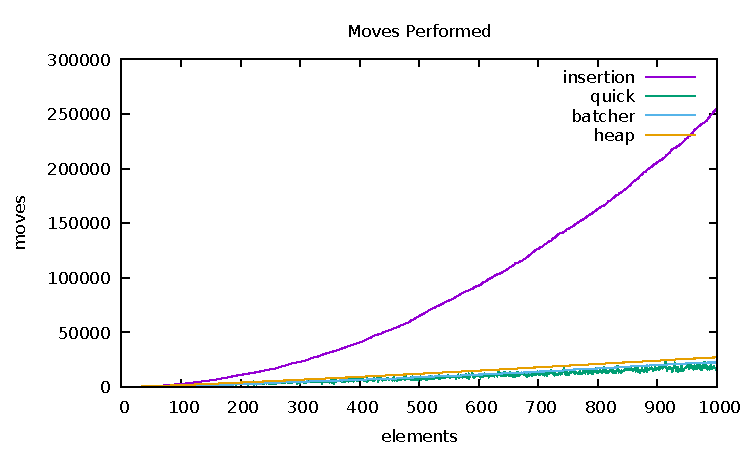
\includegraphics[width = 0.75\textwidth]{fig/length_to_moves.pdf}

In the graph above, each sorting algorithm is plotted with its number of moves on the y axis and the length of the array on the x axis. With an array length of 100 or less, each of the sorting methods seem to use a similar amount of moves. When the sorting algorithms have to sort more than 100 elements, it seems the Insertion sort algorithm runs with many more moves than the other sorting algorithms. You can also see that the Quick sort line is not straight, and it curves a lot but stays in the general vicinity of the Batcher and Heap sort lines. This is most likely because the number of comparisons and ways that Quicksort breaks up the partitions varies depending on the sorted nature of the array it is given. If the partition is already sorted then the algorithm can skip over a given partition and it could have a shorter or longer amount of moves based on the other partitions, whereas the other sorts continuously compare and move elements in the array.

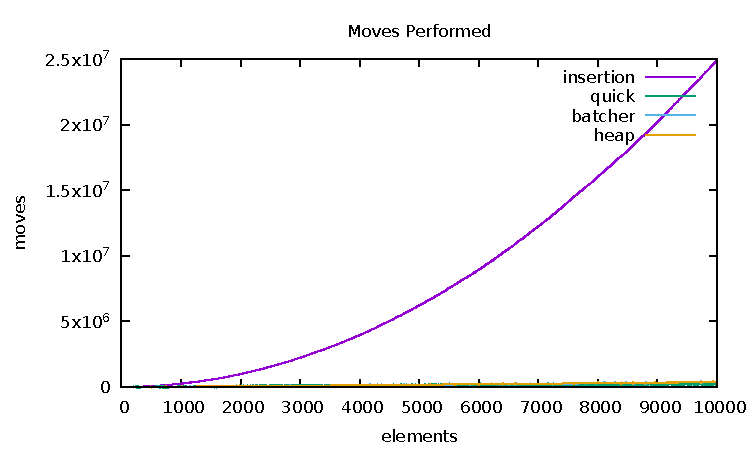
\includegraphics[width = 0.75\textwidth]{fig/larger_moves.pdf}

This figure above shows the same algorithms compared with moves and elements as above, but it uses 10000 elements instead to give a larger array size to graph. The graph with more elements shows that even with larger and larger arrays, the only one of these sorting algorithms that uses much more moves than any of the other algorithms is the Insertion sort, making it seem like this is the least efficient sort for any array above length 100.

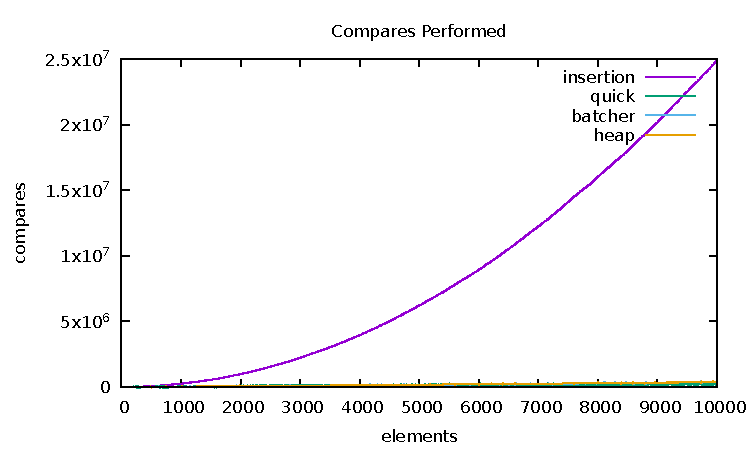
\includegraphics[width = 0.75\textwidth]{fig/length_to_compares.pdf}

The above figure shows the same sorting algorithms but it is comparing the length of the arrays to the amount of compares each algorithm uses. The graphs look very similar and the data for each are close to each other in values. This reinforces our findings that Insertion sort is the most inefficient of the 4 sorting methods.

\section{other comments}\label{ss:comments}
I followed the python pseudocode for the implementation of the sorting algorithms, and in order to use the stats and set code that we were given I watched Eugene and Omar's lab sections for better understanding about the given code and the sorts themselves. Much of my sorting.c code when it comes to using malloc() and free() come from Eugene's explanations of these commands in his lab section.

\end{document}
